\documentclass[letterpaper,12pt]{article}
\usepackage{tabularx} % extra features for tabular environment
\usepackage{amsmath}  % improve math presentation
\usepackage{float}
\usepackage{pdfpages}
\usepackage{steinmetz}

\usepackage{graphicx} % takes care of graphic including machinery
\graphicspath{ {./figures/} }
\usepackage[margin=1in,letterpaper]{geometry} % decreases margins
\usepackage{cite} % takes care of citations
\usepackage[final]{hyperref} % adds hyper links inside the generated pdf file
\hypersetup{
	colorlinks=true,       % false: boxed links; true: colored links
	linkcolor=blue,        % color of internal links
	citecolor=blue,        % color of links to bibliography
	filecolor=magenta,     % color of file links
	urlcolor =blue         
}




\begin{document}

\title{Experiment 7 Preliminary Work \protect\\ Active Filters}
\author{Ahmet Akman 2442366 \protect\\}
\date{\today}
\maketitle
\tableofcontents
%\begin{abstract}
%abstract
%\end{abstract}

%\section{Introduction}
\section{Step 1}
In this step the circuit given in Figure 1 is examined.
\begin{figure}[H]
    \centering
    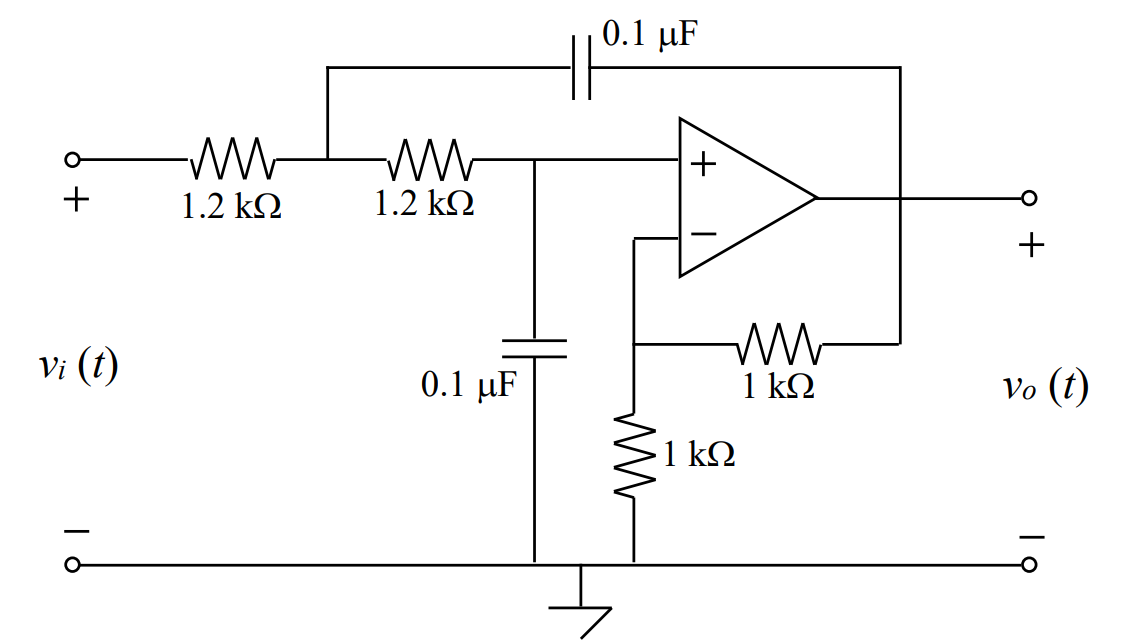
\includegraphics[width=1\textwidth]{fig1.png}
    \caption{Circuit schematic for the step 1}
\end{figure} 
\section{Step 2}
\begin{figure}[H]
\centering
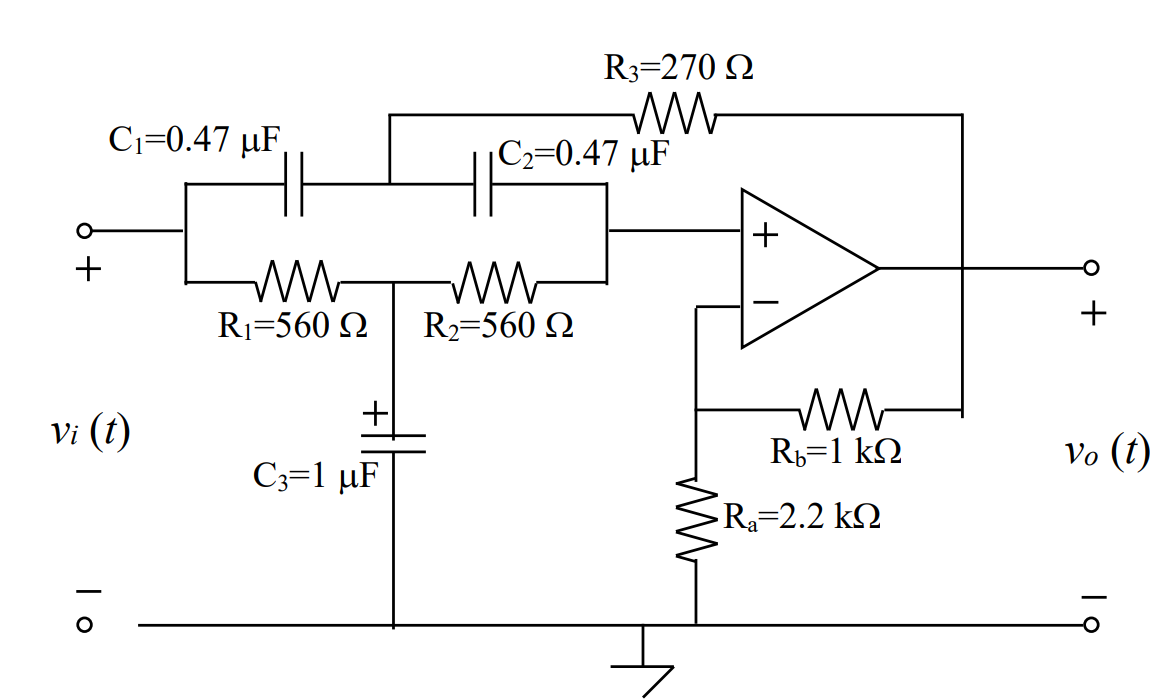
\includegraphics[width=1\textwidth]{fig2.png}
\caption{Circuit schematic for the step 2}
\end{figure} 
\section{Step 3}
\begin{figure}[H]
    \centering
    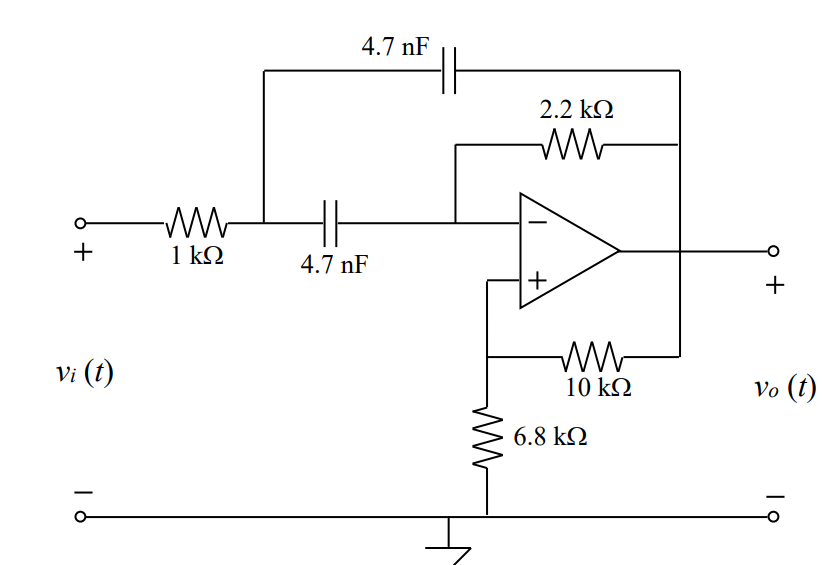
\includegraphics[width=1\textwidth]{fig3.png}
    \caption{Circuit schematic for the step 3}
\end{figure} 
\section{Simulations}
\subsection*{a}
The circuit given in Figure 1 is constructed in LTSpice environment as shown in Figure 4.
\begin{figure}[H]
    \centering
    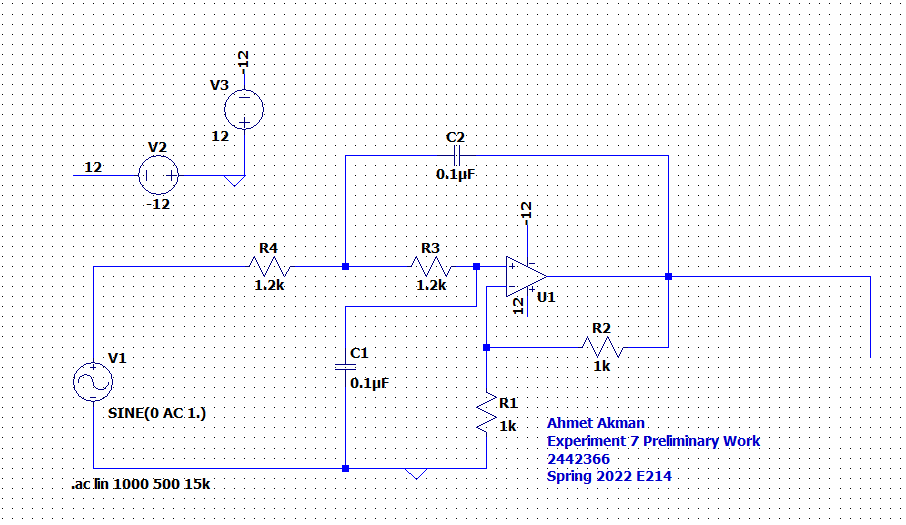
\includegraphics[width=1\textwidth]{fig1sim.png}
    \caption{Circuit simulation schematic}
\end{figure} 

As a result the magnitude response is obtained and plotted as given in Figure 5.


\begin{figure}[H]
    \centering
    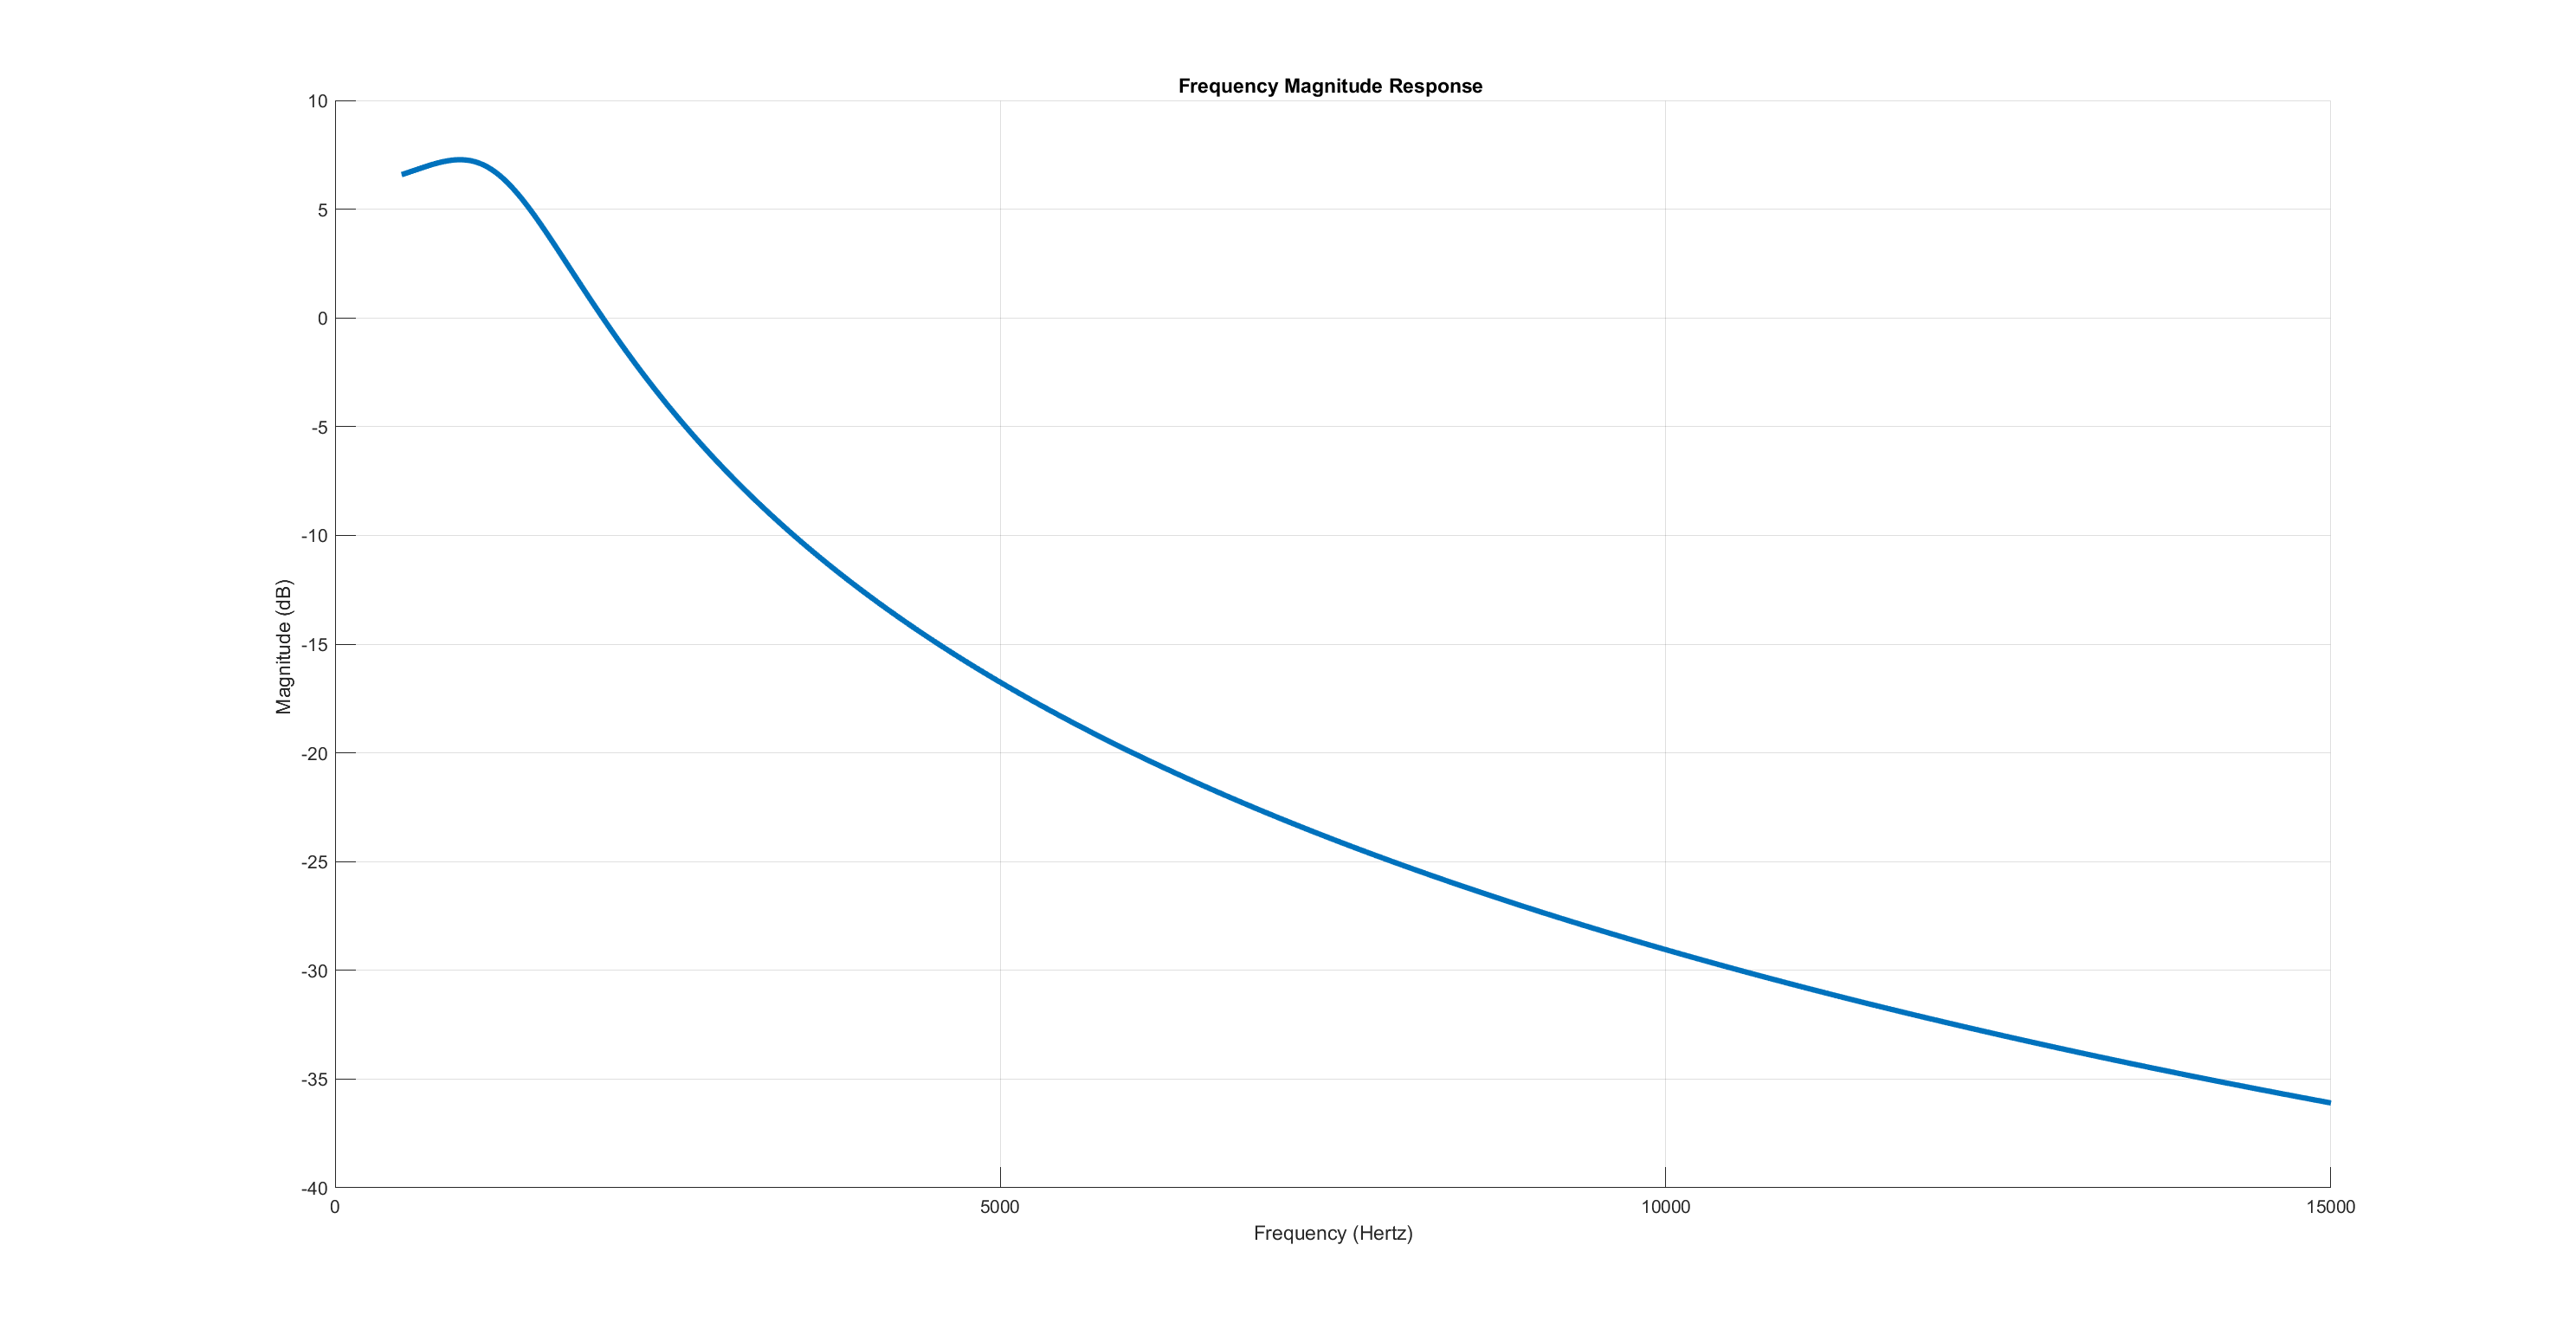
\includegraphics[width=1\textwidth]{1_1_1.png}
    \caption{Magnitude response of the circuit}
\end{figure}
It can be said that the circuit indeed functions as a low pass filter.
\subsection*{b} 
The circuit given in Figure 3 is constructed in LTSpice environment as shown in Figure 6.
\begin{figure}[H]
    \centering
    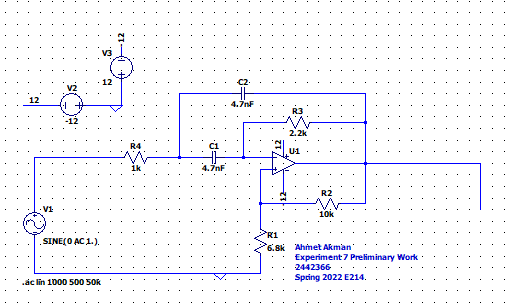
\includegraphics[width=1\textwidth]{fig3sim.png}
    \caption{Circuit simulation schematic }
\end{figure} 

As a result the frequency magnitude response given in Figure 7 is obtained.
\begin{figure}[H]
    \centering
    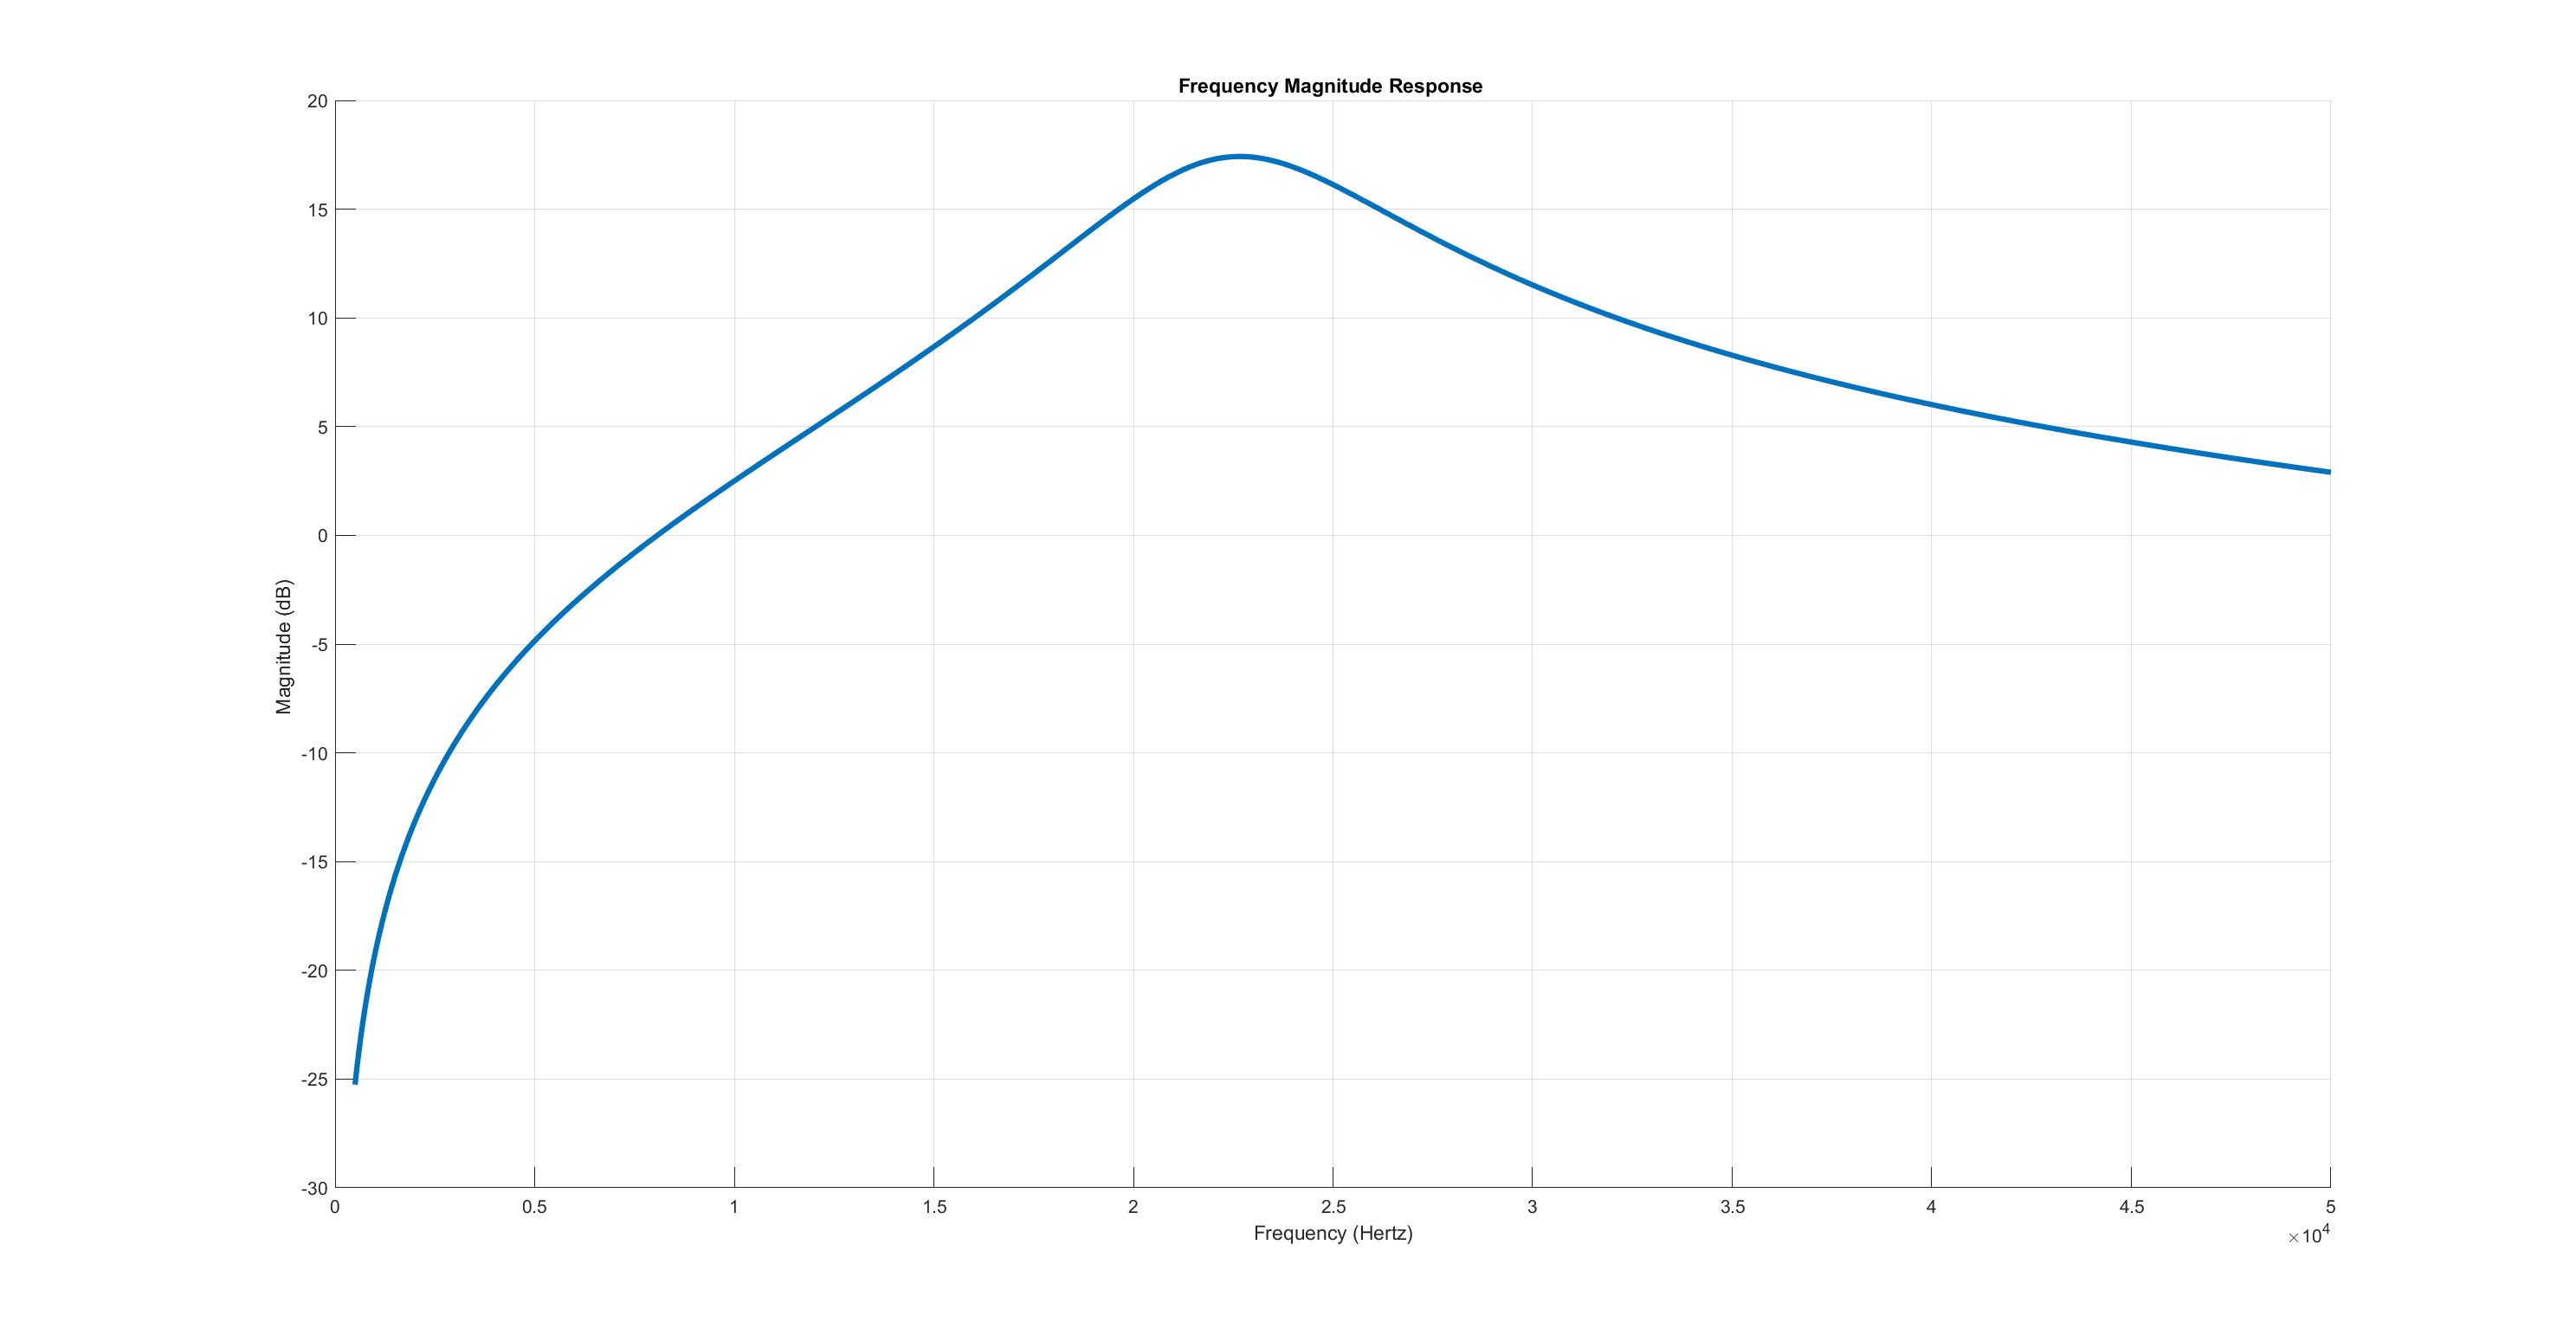
\includegraphics[width=1\textwidth]{2_1_1.png}
    \caption{Magnitude response of the circuit}
\end{figure} 

After removing the 10k and 6.8k resistors and connecting the positive terminal of the opamp to ground the response shown in Figure 8 is obtained.

\begin{figure}[H]
    \centering
    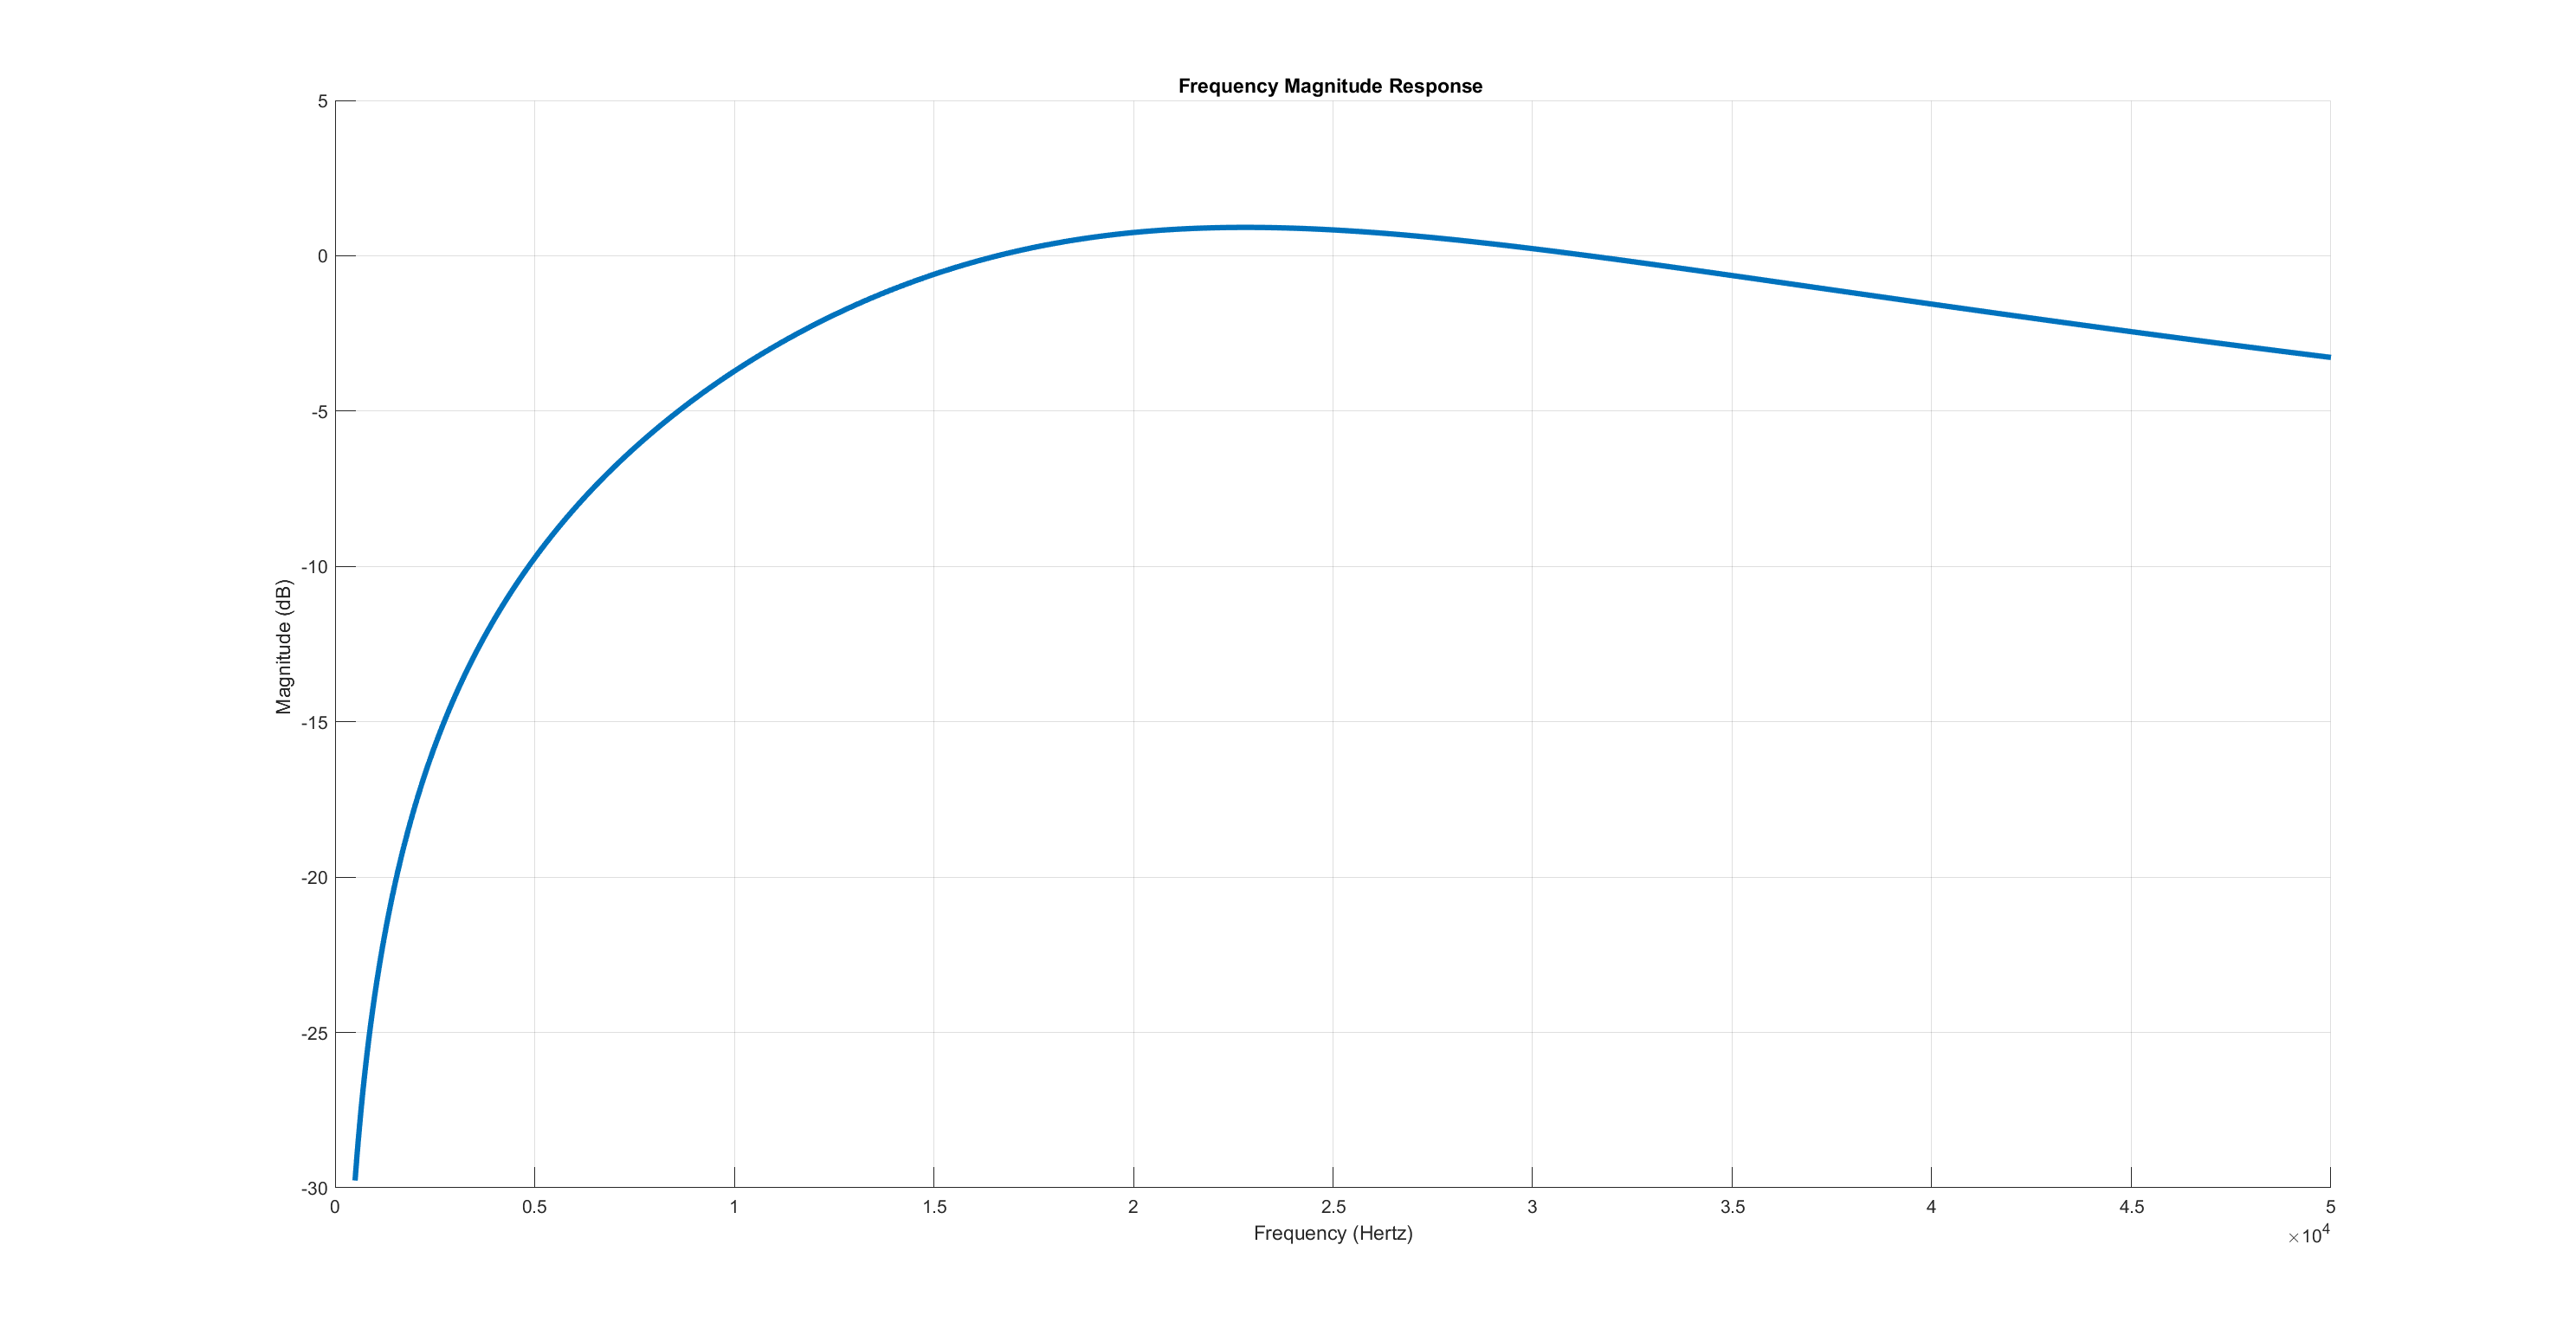
\includegraphics[width=1\textwidth]{2_1_2.png}
    \caption{Magnitude response of the circuit (the resistors are removed)}
\end{figure} 
As a result it can be said that the removal of the resistors costs the high frequency filtering ability of the circuit. On the other hand the in this setup the circuit has no or quite less gain. 

\section{Conclusion}
In this document, the preliminary work simulation results of the Experiment 7 are presented.
\section*{Appendix A}
The results of the simulations are fetched from LTSpice and plotted in MATLAB in order to make the plots more readable and convenient.


\end{document}

%%%%%%%%%%%%%%%%%%%%%%   EXAMPLE TABLE   %%%%%%%%%%%%%%%%%%%%%%%%%%%%%%%%
\begin{table}[H]
\begin{center}
    \caption{Resistance reading by color code convention.}
    \vspace{2mm}
    \begin{tabular}{||c | c | c||} 
        \hline
        Color Order & Value & Tolerance \\ [0.5ex] 
        \hline\hline
        Brown / Black / Red / Gold & 1k\( \Omega \) & \( \% \) 5  \\ 
        \hline
        Yellow / Violet / Red / Gold & 4.7k\( \Omega \) & \( \% \) 5   \\
        \hline
        Brown / Grey / Orange / Gold & 18k\( \Omega \) & \( \% \) 5  \\ [1ex] 
        \hline
    \end{tabular}
\end{center}
\end{table}


%%%%%%%%%%%%%%%%%%%%%%   EXAMPLE IMAGE   %%%%%%%%%%%%%%%%%%%%%%%%%%%%%%%%
\begin{figure}[H]
\centering
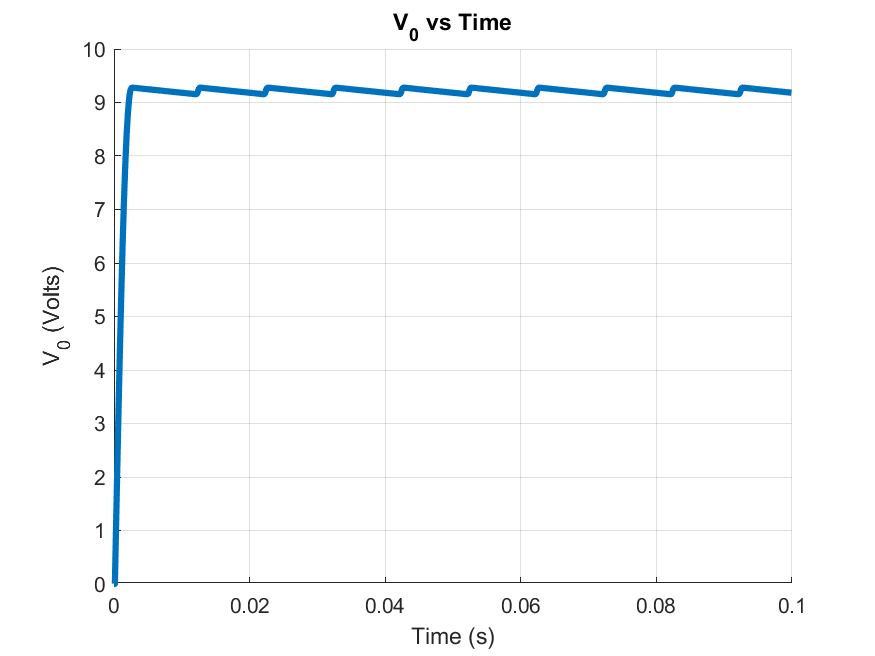
\includegraphics[width=1\textwidth]{5.png}
\caption{Circuit schematic for the step 5}
\end{figure} 

%%%%%%%%%%%%%%%%%%%%%%   EXAMPLE IMAGE FROM PDF   %%%%%%%%%%%%%%%%%%%%%%%%%%%%%%%%
\begin{figure}[H] \centering{
	\includegraphics[scale=0.25]{2a_plot.pdf}}
	\caption{Experiment 2}
\end{figure}
	